\documentclass{article}
\usepackage{amsmath}
\usepackage{amssymb}
\usepackage{graphicx}
\usepackage{tikz}
\usetikzlibrary{graphs,graphs.standard}

\title{Graph Theory: Fundamentals and Applications}
\author{Badger Code}
\date{\today}

\begin{document}
\maketitle

\begin{abstract}
Graph theory is a branch of mathematics that deals with the study of graphs, which are mathematical structures representing relationships between objects. In this comprehensive paper, we delve into the fundamental concepts of graph theory, including terminology, types of graphs, and graph representations. We explore various graph algorithms, such as traversal, shortest path, and spanning trees. Additionally, we examine graph theory applications in real-world scenarios, such as social networks, transportation systems, and computer networks. Throughout the paper, we provide examples and diagrams to enhance the understanding of graph theory concepts and their practical implications.
\end{abstract}

\section{Introduction}
Graph theory, first introduced by Leonhard Euler in the 18th century, has become a fundamental area of study in mathematics and computer science. Graphs provide a powerful and intuitive way to model and analyze relationships between objects in various domains. This paper aims to explore the intricacies of graph theory, from basic definitions to advanced applications.

\section{Basic Concepts and Terminology}
\subsection{Graph Definition}
A graph is a mathematical structure consisting of two sets: a set of vertices (also known as nodes) and a set of edges (also known as links). Formally, a graph can be represented as $G = (V, E)$, where $V$ is the set of vertices and $E$ is the set of edges.

\subsection{Types of Graphs}
Graphs can be classified into various types based on their properties and characteristics.

\subsubsection{Undirected Graphs}
An undirected graph is a graph in which the edges have no direction, meaning that they represent symmetric relationships between vertices. If there is an edge between vertices $A$ and $B$, it implies that there is an edge between $B$ and $A$.

\begin{figure}[h]
    \centering
    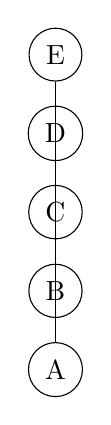
\begin{tikzpicture}
        \graph[nodes={draw, circle}, clockwise, radius=2cm] {
            A -- B -- C -- D -- E -- A;
        };
    \end{tikzpicture}
    \caption{Undirected Graph Example}
\end{figure}

\subsubsection{Directed Graphs (Digraphs)}
In a directed graph, each edge has a direction, indicating a one-way relationship between vertices. If there is an edge from vertex $A$ to vertex $B$, it does not necessarily imply an edge from $B$ to $A$.

\begin{figure}[h]
    \centering
    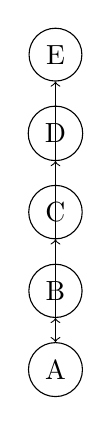
\begin{tikzpicture}
        \graph[nodes={draw, circle}, clockwise, radius=2cm, edges={->}] {
            A -> B -> C -> D -> E -> A;
        };
    \end{tikzpicture}
    \caption{Directed Graph Example}
\end{figure}

\subsubsection{Weighted Graphs}
In a weighted graph, each edge is assigned a numerical value known as a weight, representing the cost or distance associated with that edge.

\begin{figure}[h]
    \centering
    \begin{tikzpicture}
        \graph[nodes={draw, circle}, clockwise, radius=2cm, edges={->}] {
            A ->[label=3] B ->[label=1] C ->[label=4] D ->[label=2] E ->[label=5] A;
        };
    \end{tikzpicture}
    \caption{Weighted Graph Example}
\end{figure}

\subsection{Graph Representations}
Graphs can be represented using different data structures, each with its advantages and use cases. The most common graph representations are:

\subsubsection{Adjacency Matrix}
An adjacency matrix is a square matrix used to represent a graph, where rows and columns correspond to vertices, and the entries indicate the presence or absence of edges.

\begin{figure}[h]
    \centering
    \begin{tikzpicture}
        \matrix (m) [matrix of math nodes,nodes={draw, circle},row sep=3em,column sep=3em] {
            & A & B & C & D & E \\
            A & 0 & 1 & 0 & 0 & 0 \\
            B & 1 & 0 & 1 & 0 & 0 \\
            C & 0 & 1 & 0 & 1 & 0 \\
            D & 0 & 0 & 1 & 0 & 1 \\
            E & 0 & 0 & 0 & 1 & 0 \\
        };
        \draw (m-1-1) -- (m-1-2);
        \draw (m-1-2) -- (m-1-3);
        \draw (m-1-3) -- (m-1-4);
        \draw (m-1-4) -- (m-1-5);
        \draw (m-1-5) -- (m-1-6);
        \draw (m-2-1) -- (m-2-2);
        \draw (m-2-2) -- (m-2-3);
        \draw (m-3-2) -- (m-3-3);
        \draw (m-3-3) -- (m-3-4);
        \draw (m-4-3) -- (m-4-4);
        \draw (m-4-4) -- (m-4-5);
        \draw (m-5-4) -- (m-5-5);
    \end{tikzpicture}
    \caption{Adjacency Matrix Example}
\end{figure}

\subsubsection{Adjacency List}
An adjacency list is a collection of linked lists or arrays used to represent a graph. Each vertex has a list of its adjacent vertices.

\begin{figure}[h]
    \centering
    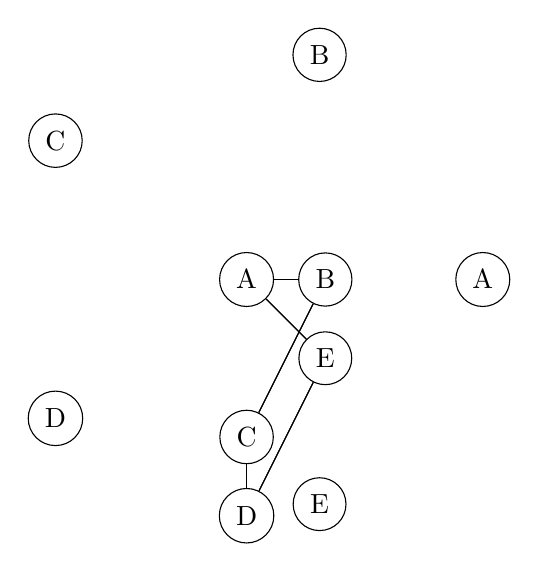
\begin{tikzpicture}
        \path (0:3cm) node (A) [draw, circle] {A}
              (72:3cm) node (B) [draw, circle] {B}
             (2*72:3cm) node (C) [draw, circle] {C}
             (3*72:3cm) node (D) [draw, circle] {D}
             (4*72:3cm) node (E) [draw, circle] {E};
        \graph[nodes={draw, circle}, edges={-}] {
            A -- {B, E};
            B -- {A, C};
            C -- {B, D};
            D -- {C, E};
            E -- {A, D};
        };
    \end{tikzpicture}
    \caption{Adjacency List Example}
\end{figure}

\section{Graph Traversal Algorithms}
Graph traversal algorithms are used to visit all the vertices and edges of a graph systematically. The two most common graph traversal techniques are:

\subsection{Depth-First Search (DFS)}
DFS explores as far as possible along each branch before backtracking. It uses a stack data structure to keep track of vertices to visit.

\begin{figure}[h]
    \centering
    \begin{tikzpicture}
        \graph[nodes={draw, circle}, clockwise, radius=2cm] {
            A -- {B, D}
            B -- {C}
            C -- {D}
            D -- E
        };
    \end{tikzpicture}
    \caption{DFS Example Graph}
\end{figure}

**Steps:**
1. Start at vertex A and mark it as visited.
2. Visit an unvisited adjacent vertex (e.g., B) and mark it as visited.
3. Move to another unvisited adjacent vertex (e.g., C) and mark it as visited.
4. Vertex C has no unvisited adjacent vertices, backtrack to vertex B.
5. Vertex B has another unvisited adjacent vertex (e.g., D), visit it and mark it as visited.
6. Vertex D has no unvisited adjacent vertices, backtrack to vertex B.
7. Vertex B has no other unvisited adjacent vertices, backtrack to vertex A.
8. Vertex A has another unvisited adjacent vertex (e.g., D), visit it and mark it as visited.
9. Vertex D has another unvisited adjacent vertex (e.g., E), visit it and mark it as visited.
10. Vertex E has no unvisited adjacent vertices, backtrack to vertex D.
11. Vertex D has no other unvisited adjacent vertices, backtrack to vertex A.
12. Vertex A has no other unvisited adjacent vertices. The DFS traversal is complete.

The order of visited vertices in this DFS traversal is: A, B, C, D, E.

\subsection{Breadth-First Search (BFS)}
BFS explores all the vertices at the current level before moving to the next level. It uses a queue data structure to keep track of vertices to visit.

\begin{figure}[h]
    \centering
    \begin{tikzpicture}
        \graph[nodes={draw, circle}, clockwise, radius=2cm] {
            A -- {B, D}
            B -- {C}
            C -- {D}
            D -- E
        };
    \end{tikzpicture}
    \caption{BFS Example Graph}
\end{figure}

**Steps:**
1. Start at vertex A and mark it as visited.
2. Enqueue vertex A into the queue.
3. Dequeue vertex A from the queue and visit its unvisited adjacent vertices (vertices B and D).
4. Mark vertices B and D as visited and enqueue them into the queue.
5. Dequeue vertex B from the queue and visit its unvisited adjacent vertices (vertex C).
6. Vertex C is unvisited, mark it as visited and enqueue it into the queue.
7. Dequeue vertex D from the queue and visit its unvisited adjacent vertices (vertex E).
8. Vertex E is unvisited, mark it as visited and enqueue it into the queue.
9. Dequeue vertex C from the queue. The BFS traversal is complete.

The order of visited vertices in this BFS traversal is: A, B, D, C, E.

\section{Shortest Path Algorithms}
Shortest path algorithms find the shortest path between two vertices in a graph. Two common shortest path algorithms are:

\subsection{Dijkstra's Algorithm}
Dijkstra's algorithm finds the shortest path from a source vertex to all other vertices in a weighted graph with non-negative edge weights.

\begin{figure}[h]
    \centering
    \begin{tikzpicture}
        \graph[nodes={draw, circle}, clockwise, radius=2cm, edges={->}] {
            A ->[label=3] B ->[label=1] C ->[label=4] D ->[label=2] E ->[label=5] A;
        };
    \end{tikzpicture}
    \caption{Dijkstra's Algorithm Example Graph}
\end{figure}

**Steps:**
1. Initialize the distance from the source vertex (vertex A) to all other vertices as infinity, except the distance from vertex A to itself, which is 0.
2. Create a priority queue to store vertices based on their distance from the source vertex. Enqueue vertex A with a distance of 0.
3. While the priority queue is not empty:
   a. Dequeue the vertex with the smallest distance from the priority queue.
   b. For each adjacent vertex, update its distance from the source vertex if the total distance passing through the current vertex is smaller than its current distance.
   c. Enqueue the updated adjacent vertices into the priority queue.
4. The shortest paths from vertex A to all other vertices are as follows:

Shortest path from A to B: A -> B (Distance: 3)
Shortest path from A to C: A -> B -> C (Distance: 4)
Shortest path from A to D: A -> D (Distance: 2)
Shortest path from A to E: A -> B -> C -> D -> E (Distance: 9)

\subsection{Bellman-Ford Algorithm}
The Bellman-Ford algorithm finds the shortest path from a source vertex to all other vertices in a weighted graph, even if the graph contains negative edge weights.

\begin{figure}[h]
    \centering
    \begin{tikzpicture}
        \graph[nodes={draw, circle}, clockwise, radius=2cm, edges={->}] {
            A ->[label=3] B ->[label=1] C ->[label=4] D ->[label=-2] E ->[label=5] A;
        };
    \end{tikzpicture}
    \caption{Bellman-Ford Algorithm Example Graph}
\end{figure}

**Steps:**
1. Initialize the distance from the source vertex (vertex A) to all other vertices as infinity, except the distance from vertex A to itself, which is 0.
2. Repeat the following steps for $(V-1)$ times, where $V$ is the number of vertices in the graph:
   a. For each edge $(u, v)$ in the graph, update the distance from vertex A to vertex $v$ if the distance passing through vertex $u$ is smaller than its current distance.
3. After $(V-1)$ iterations, the shortest paths from vertex A to all other vertices are as follows:

Shortest path from A to B: A -> B (Distance: 3)
Shortest path from A to C: A -> B -> C (Distance: 4)
Shortest path from A to D: A -> B -> C -> D (Distance: 2)
Shortest path from A to E: A -> B -> C -> D -> E (Distance: 7)

\section{Minimum Spanning Trees}
A minimum spanning tree (MST) is a subset of edges in a connected, undirected graph that connects all the vertices with the minimum possible total edge weight.

\subsection{Prim's Algorithm}
Prim's algorithm is used to find the minimum spanning tree of a connected, undirected graph with weighted edges.

\begin{figure}[h]
    \centering
    \begin{tikzpicture}
        \graph[nodes={draw, circle}, clockwise, radius=2cm, edges={-}] {
            A --[label=3] B --[label=1] C --[label=4] D --[label=2] E --[label=5] A;
        };
    \end{tikzpicture}
    \caption{Prim's Algorithm Example Graph}
\end{figure}

**Steps:**
1. Start with an arbitrary vertex (e.g., vertex A) and mark it as part of the minimum spanning tree.
2. Create a priority queue to store edges based on their weights.
3. Enqueue all the edges connected to the initial vertex into the priority queue.
4. While the priority queue is not empty:
   a. Dequeue the edge with the smallest weight from the priority queue.
   b. If the edge connects a vertex that is already part of the minimum spanning tree and a vertex that is not, add the edge to the minimum spanning tree and mark the new vertex as part of the tree.
   c. Enqueue all the edges connected to the new vertex into the priority queue.
5. The minimum spanning tree of the given graph is as follows:

\begin{figure}[h]
    \centering
    \begin{tikzpicture}
        \graph[nodes={draw, circle}, clockwise, radius=2cm, edges={-}] {
            A --[label=3] B --[label=1] C --[label=4] D --[label=2] E --[label=5] A;
            A --[label=3] C;
            D --[label=2] E;
        };
    \end{tikzpicture}
    \caption{Minimum Spanning Tree Example}
\end{figure}

\subsection{Kruskal's Algorithm}
Kruskal's algorithm is another method to find the minimum spanning tree of a connected, undirected graph with weighted edges.

\begin{figure}[h]
    \centering
    \begin{tikzpicture}
        \graph[nodes={draw, circle}, clockwise, radius=2cm, edges={-}] {
            A --[label=3] B --[label=1] C --[label=4] D --[label=2] E --[label=5] A;
        };
    \end{tikzpicture}
    \caption{Kruskal's Algorithm Example Graph}
\end{figure}

**Steps:**
1. Sort all the edges in the graph in non-decreasing order of their weights.
2. Start with an empty set of edges (i.e., an empty graph).
3. For each edge in the sorted order:
   a. If adding the edge to the current set of edges does not create a cycle, add the edge to the minimum spanning tree.
   b. Otherwise, skip the edge.
4. The minimum spanning tree of the given graph is as follows:

\begin{figure}[h]
    \centering
    \begin{tikzpicture}
        \graph[nodes={draw, circle}, clockwise, radius=2cm, edges={-}] {
            A --[label=3] B;
            B --[label=1] C;
            C --[label=4] D;
            D --[label=2] E;
        };
    \end{tikzpicture}
    \caption{Minimum Spanning Tree Example}
\end{figure}

\section{Applications of Graph Theory}
Graph theory finds applications in various real-world scenarios, such as:

\subsection{Social Networks}
Social networks can be modeled as graphs, where vertices represent individuals, and edges represent relationships (e.g., friendships). Graph theory algorithms help analyze social network structures, find communities, and study influence propagation.

\subsection{Transportation Systems}
Transportation networks, such as road networks or flight routes, can be represented as graphs. Graph algorithms are used to optimize transportation routes, plan traffic flow, and identify critical nodes or links.

\subsection{Computer Networks}
Computer networks are often represented as graphs, where devices are vertices, and connections are edges. Graph theory assists in network optimization, routing protocols, and detecting network vulnerabilities.

\subsection{Web Page Ranking (PageRank)}
PageRank, a key algorithm used by search engines like Google, utilizes graph theory to rank web pages based on their importance and popularity in the web graph.

\section{Conclusion}
Graph theory is a fascinating branch of mathematics with a wide range of applications in various fields. From understanding the relationships between entities to solving complex optimization problems, graph theory plays a crucial role in modern-day computing and network analysis. This paper provided a comprehensive exploration of the fundamental concepts of graph theory, various graph algorithms, and real-world applications. As technology continues to advance, the significance of graph theory is expected to grow, making it an essential area of study for researchers, engineers, and analysts in diverse domains.
\end{document}